\documentclass[a4paper,11pt]{report}
\usepackage[T1]{fontenc}
\usepackage[utf8]{inputenc}
\usepackage{lmodern}
\usepackage[english]{babel}
\usepackage[siunitx, american, smartlabels, cute inductors, europeanvoltages]{circuitikz}
\usepackage{multirow}
\usepackage{subfig}
\usepackage{amsmath}



\title{NEXT - Energy Plane Status Report }
\author{Vicente Herrero, Juanjo Gomez-Cadenas, Raul Esteve, Vicente Álvarez}

\begin{document}

\maketitle
\tableofcontents

\begin{abstract}
Front End Electronics (FEE) and complementary Digital Signal Processing (DSP) techniques will be described in this report. Also data measurements taken in order to verify FEE behavior and validate DSP techniques will be presented. Finally some conclusions will be introduced as well as possible future work lines
\end{abstract}

\chapter{Grounded Cathode PMT Connection and its Consequences}
\par In order to simplify Energy Plane construction and integration in the vessel structure, PMT enclosure and thus its cathode connection are directly connected to the vessel copper mass. This fact implies that a \textbf{PMT grounded cathode connection scheme} must be used since the whole structure must be connected to earth for electrical safety reasons.



\section{Grounded Cathode PMT Connection}

\par In such a configuration the anode output must be AC coupled through an isolation capacitor since anode output DC voltage equals the high voltage (HV) being applied to the PMT (fig. \ref{fig:grounded_cathode}). As a consequence the AC coupling capacitor must be able to withstand the HV needed to provide the required gain in the PMT (typically from 1000 V to 2000 V). 

\begin{figure}
  \begin{center}
    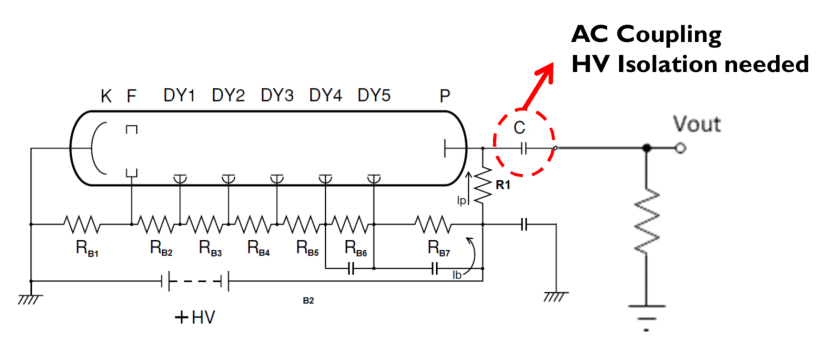
\includegraphics[width=\textwidth]{./figures/grounded_cathode.pdf}
    \caption{Grounded Cathode PMT connection scheme}
    \label{fig:grounded_cathode}
  \end{center}
\end{figure}

Moreover the use of an AC coupling scheme implies a high pass filter (HPF) will be created. Such a filter blocks or attenuates a range of frequencies from DC up to a certain frequency \textit{(cutoff frequency)}. Figure \ref{fig:GC_equivalent_circuit} shows the electrical equivalent circuit of this connection scheme as well as its frequency response whose Laplace transfer function is shown in eq. \ref{eq:1}


\begin{figure}
\begin{center}$
\begin{array}{cc}
  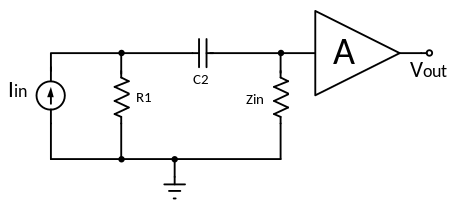
\includegraphics[width=0.5\textwidth]{./figures/FEE_simple.png} &
  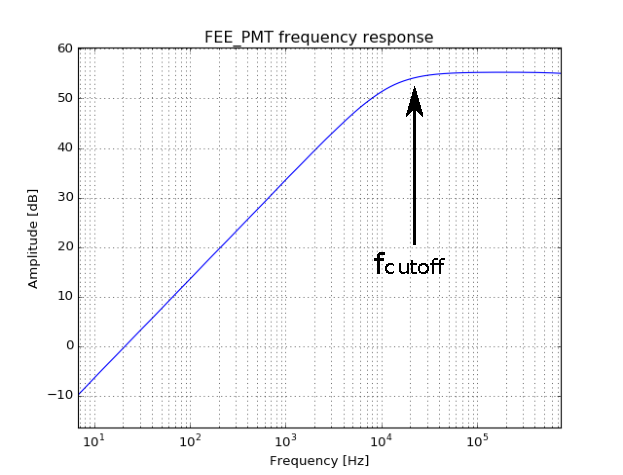
\includegraphics[width=0.5\textwidth]{./figures/FEEsimple_freq_response.pdf}
\end{array}$
\end{center}
\caption{Grounded Cathode Equivalent Circuit and Frequency response}
\label{fig:GC_equivalent_circuit}
\end{figure}


\begin{equation}
\frac{v_O}{i_I}=A\frac{Z_{in}R_1}{Z_{in}+R_1}\frac{(R_1+Z_{in})Cs}{1+(R_1+Z_{in})Cs}
\label{eq:1}
\end{equation}

\begin{equation}
f_{cutoff}=\frac{1}{(R_1+Z_{in})C.2\pi}
\end{equation}

From the time domain point of view, the AC coupling effect wipes out the DC component on the signal. As a consequence a distortion is introduced that makes difficult to get an estimation of the energy of a complex signal based on its area. Figure \ref{fig:pulses} shows the AC coupling effect on a single pulse and a complex signal. In the latter case the total negative and positive area computation predicts a lower number of pulses (2.28 instead of 3). The baseline shift effect must be corrected if a high resolution measurement is needed. Two possible solutions will be explain in the next section.

\begin{figure}
\begin{center}$
\begin{array}{cc}
  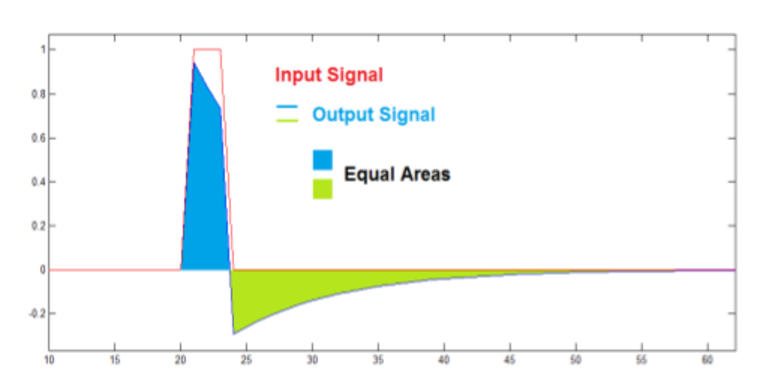
\includegraphics[width=0.5\textwidth]{./figures/pulse.pdf} &
  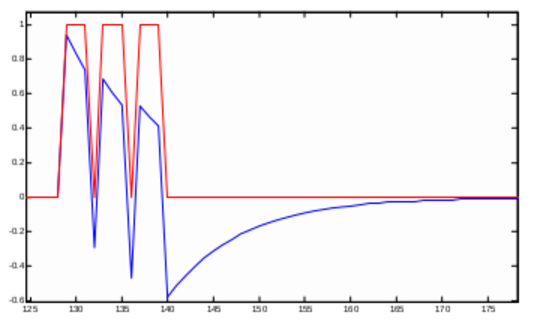
\includegraphics[width=0.5\textwidth]{./figures/pulses.pdf}
\end{array}$
\end{center}
\caption{AC coupling effect on Energy Estimation}
\label{fig:pulses}
\end{figure}


\subsection{High $\tau$ constant value solution}
Since the $\tau$ of the equivalent circuit shown in fig. \ref{fig:grounded_cathode} equals the inverse of $f_{cutoff}$, a higher $\tau$ will attenuate a shorter range of frequencies producing a signal which closely resembles the original one (fig. \ref{fig:BIG_RC}). However there is a problem with the implementation of this solution. Good quality AC coupling capacitors that can withstand high voltages typically have low nominal values. It is hard to find capacitors higher than \textbf{\textit{10 nF}} that meet such specifications. Then high value resistors must be used. The example below shows how to compute the resistor value needed as a function of the signal loss in amplitude which has a direct effect on energy resolution.

\begin{figure}
  \begin{center}
    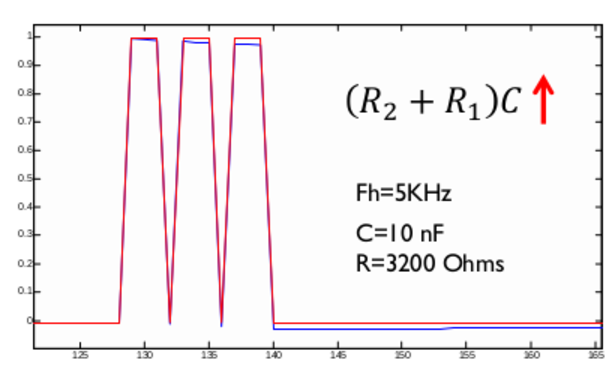
\includegraphics[width=0.6\textwidth]{./figures/BIG_RC}
    \caption{Effect of high value $\tau$ constant}
    \label{fig:BIG_RC}
  \end{center}
\end{figure}

\begin{description}
  \item[C value as a function of Baseline Shift]
The baseline shift due to voltage change in AC coupling capacitor can be computed as the charge and discharge voltage across its terminals due to a signal change in the input. The charge / discharge curve of a capacitor is related to its $\tau$ in the circuit and follows eq. \ref{eq:2} where $\tau=\frac{1}{(R_1+Z_{in})C}$.
\begin{equation}
\Delta V_C=V_C.(1-e^{-t\tau})
\label{eq:2}
\end{equation}
For a $\Delta V_C = 0.25\%$ of $V_C$ which would translate approximately into a $0.5\%$ energy resolution error and pulses of a length about $200\mu s$ the minimum allowable resistor value for a \textbf{10 nF} capacitor equals \textbf{8 M$\Omega $}
This means that for better energy resolution measurements higher resistor values would be desirable (at least 15 M$\Omega $ would be  recommended)
\end{description}

Such high value resistors introduce thermal noise issues which should be carefully studied. Since this thermal noise gets filtered by the rest of the circuit that comprises the AC coupling capacitor $C$ and $R_1$ the equivalent noise power should be low. However it will have a strong low frequency weight that could translate into additional baseline shifts. Anyway noise is not the most important issue when dealing with such high value resistors. The isolation from HV can be affected depending on effective DC resistance of the capacitor. Also Dissipation Factor of the capacitor effect might play a significant role.
\begin{description}
    \item[AC coupling capacitor Dissipation Factor effect] 
    The parallel parasitic resistance ($R_{par}$) of the AC coupling capacitor works as a by-pass path for signals in the LF frequency range (fig. \ref{fig:RPAR}. The integral of the AC coupled signal should be zero for an ideal capacitor but it isn't so. There is a small amount of positive (for a positive pulse) offset at the end of the pulse. The origin of this offset is in the part of the input signal which by-passes the coupling capacitor through the parasitic resistance. The final value of the integral at the end of the signal is the whole error we expect in the final energy calculation due to non-ideality of the capacitor.
    
    \begin{figure}
      \begin{center}
        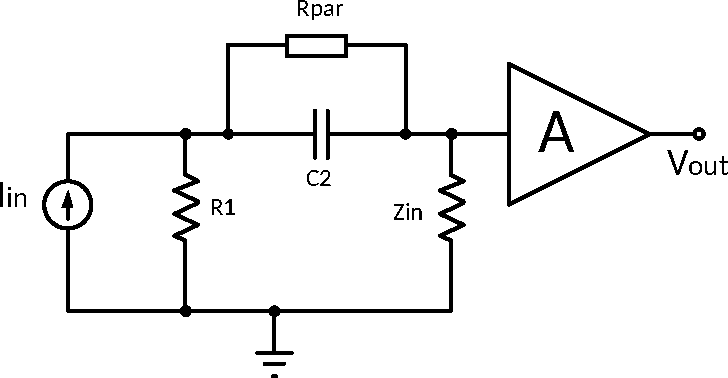
\includegraphics[width=0.5\textwidth]{./figures/RPAR_effect}
        \caption{AC coupling capacitor RPAR effect}
        \label{fig:RPAR}
      \end{center}
    \end{figure}
    
    The value of the $R_{par}$ based on datasheet values (DF=0.15\%) and assuming that the characteristics of CG0 capacitors being used remain unchanged for all the voltage range can be computed with eq. \ref{eq:3}. Finally $R_{par}$ has a value of \textbf{10 M$\Omega$}
    \begin{equation}
    DF = \frac{ESR}{Z_c} // 
    Z_c = \frac{1}{2.\pi.f.C} //
    Q = \frac{1}{DF} //
    R_{par} = Q^{2}(ESR) 
    \label{eq:3}
    \end{equation}
  \end{description}  

  As a result of this $R_{par}$ value, low frequency components of the input signal (signal pulses can be really long, up to 200 $\mu s$) as well as low frequency noise coupled to the connection cables would be translated to the output with almost none attenuation \footnote{Zero introduced by RPAR ($\frac{1}{R_{par}.C}$) would be close to the dominant pole of the circuit ($\frac{1}{(R_{par}//Zin.C}$) }. SPICE simulations has been carried out in order to measure this effect. For 200$\mu s$ length pulses the error in area estimation would be about \textbf{0.20\%} due to this effect, which should be added to the maximum baseline shift established by the capacitor value.


\chapter{Front End Electronics Design}

  A simplified version of the FEE is shown in fig. \ref{fig:FEE_scheme}. A pseudo-differential transmission has been chosen in order to reduce coupled noise which is expected to be high, since the distance between the FEE rack and the vessel is about 12 meters. The AC coupled transmission allows to inject high voltage supply to the PMTs through the same signal cable. Since C1 AC coupling capacitors will have a better frequency response and higher SFR, the line termination ($120\Omega$) will be implemented at Zin which will have a value of $60\Omega$. This option also allows to terminate the common mode signal that travels along the transmission line and is expected to be quite high since a non fully differential transmission is being used. The common mode termination is implemented at the amplifier input ($\pi$ type termination is used, as seen in \ref{fig_FEE_full}).
  
  R1 will be the high value resistor which will form a high $\tau$ constant with C1. The base stabilization C2 and C3 capacitors must have a high value to keep a good linearity in the PMT. Other mirror capacitors will be placed in the PMT base inside the vessel (not shown). The base design is a standard RC chain with the voltage values recommended by Hamamatsu. Radiopurity specs must be accomplished for every part inside the vessel.


\begin{figure}
  \begin{center}
    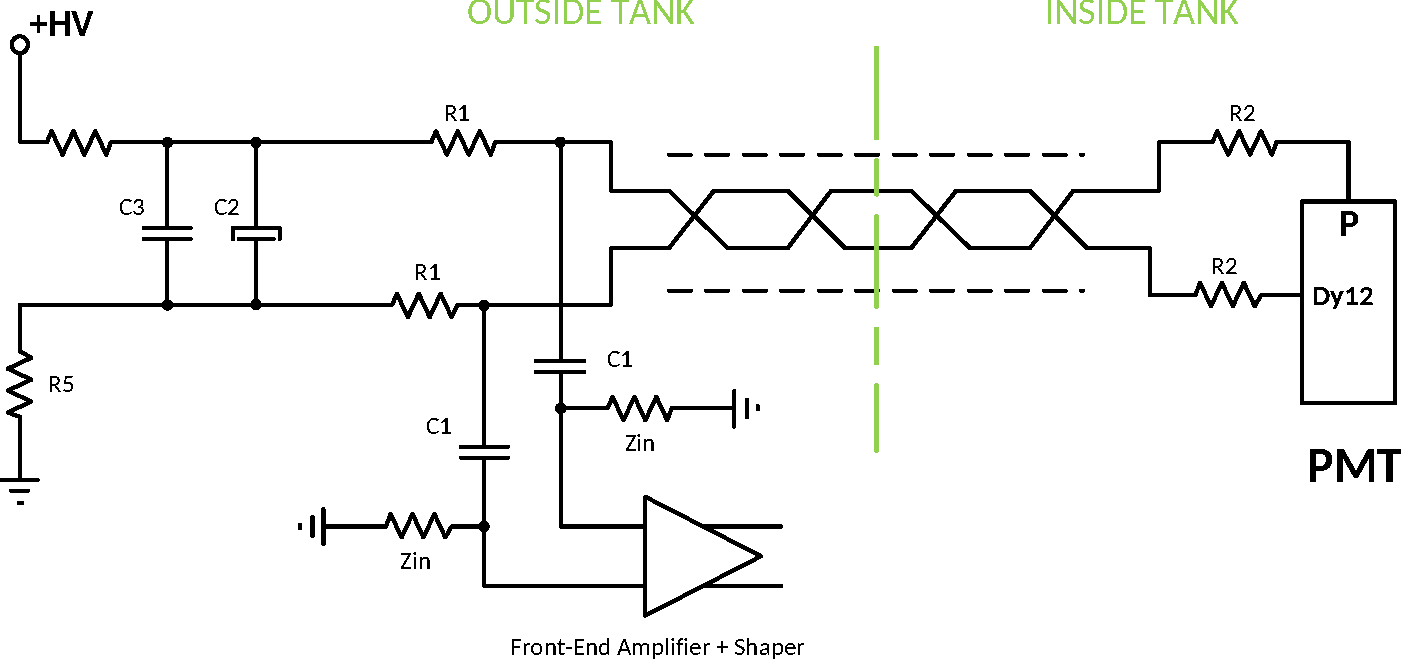
\includegraphics[width=\textwidth]{./figures/FEE_simple_scheme.pdf}
    \caption{Simplified FEE Scheme}
    \label{fig:FEE_scheme}
  \end{center}
\end{figure}

\begin{figure}
  \begin{center}
    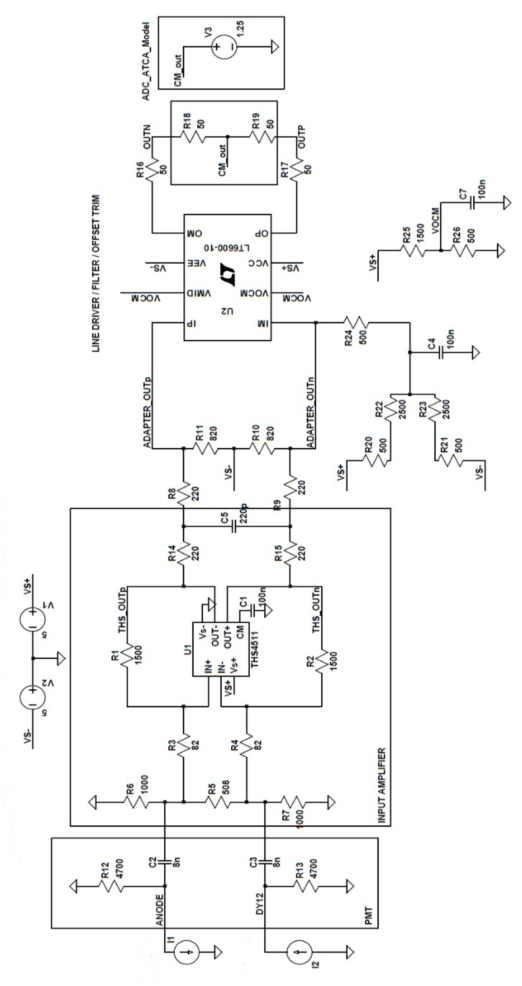
\includegraphics[width=0.8\textwidth]{./figures/FEE_full.pdf}
    \caption{}
    \label{fig:fig_FEE_full}
  \end{center}
\end{figure}


\section{Digital Baseline Restoring alternative}
Our proposal for this novel FEE design is to reduce the value of the R1 resistor. This would bring a wide swing in the baseline but it can be accurately recovered using a Digital Signal Processing algorithm once the AC coupled signal has been acquired. The decision has been taken based on the results shown in the previous section: extremely high resistor values gave results close to the energy resolution limits, and second order effects related to components parasitics might have a strong influence on final results. Moreover high impedance nodes always show a bad behavior when dealing with coupled external noise. As a result a trade-off between low frequency effects suppression and feasibility of signal recovery has been established. The lower the $f_{cutoff}$ the easier to recover the AC coupled signal but the higher the vulnerability to low frequency noise and baseline random walks that can have a very negative effect on energy resolution computation in long signals. A value of R1=$1600\Omega$ has been chosen which gives a $f_{cutoff}$ = 10 kHz. This should attenuate most of the common noises related to electrical engines and other industrial environment elements. Higher $f_{cutoff}$ frequencies would provide a better filtering effect but also would reduce SNR due to the loss in signal amplitude in AC coupled signals.
\par Figure \ref{fig:design_facts} shows some of the specifications used in the FEE design. Noise has been one of the most important specs, carefully studied from the beginning in order to enhance energy resolution results. The active components in the FEE have been chosen mainly relying on their noise specs. 
\par The bandwidth of the FEE (3MHz) has been chosen to make it work as a shaping filter, stretching the time length of the single foto-electron response that was provided as a specification by the detector calibration team.

\par In the last FEE version which will be installed by the end of the year ESD protections will be enhanced since many HV events have been detected which come close to the limits of the actual protection elements. Anyway no damage due to ESD has been recorded up to now. 

\par A rework was required to adapt FEE output common mode to ATCA input common mode as the difference between them introduced an overload and an excessive power consumption at the FEE output line driver. 


\begin{figure}
  \begin{center}
    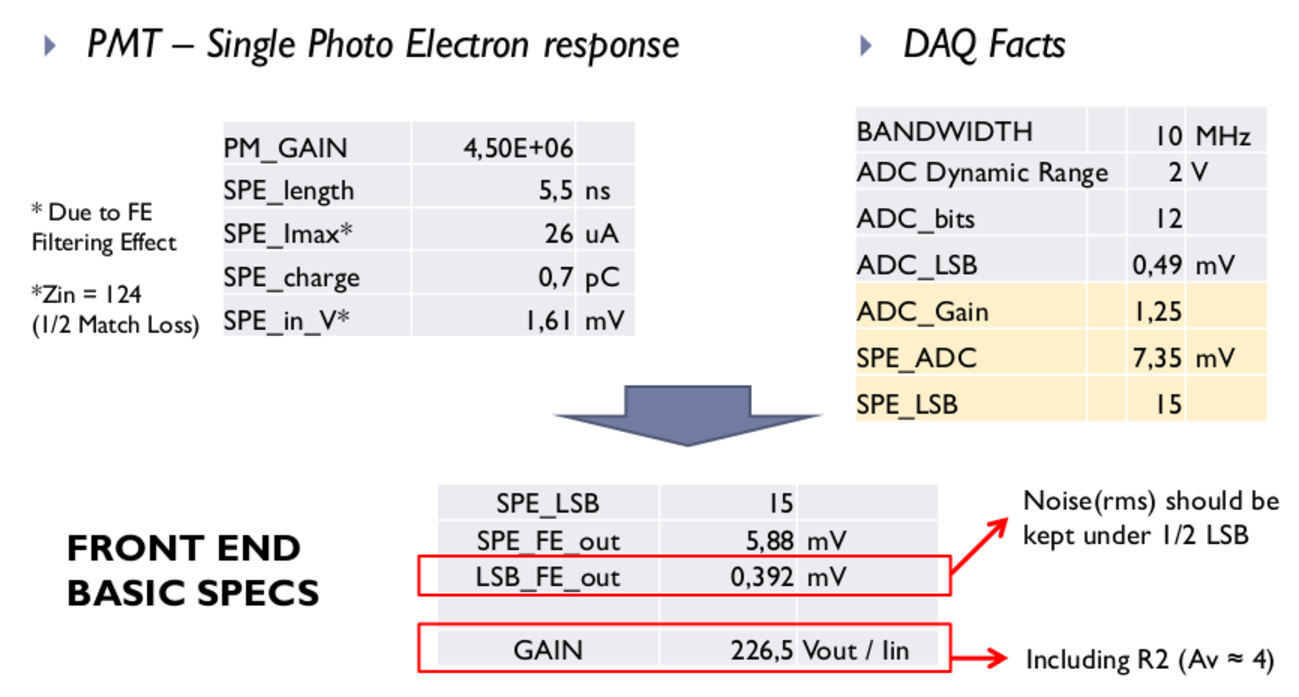
\includegraphics[width=\textwidth]{./figures/design_facts.pdf}
    \caption{}
    \label{fig:design_facts}
  \end{center}
\end{figure}
 
  
\section{Noise Measurements}
In order to check the specs of the design, noise measurements have been carried out in the laboratory and at the LSC NEXT installation. The results are shown in the table \ref{tab:noise}. 
  \begin{table}
    \caption{Noise Measurements (in $LSB_{rms}$)}
    \label{tab:noise}
  
    \begin{center}
      \begin{tabular}{ c c || c | c |}
       & & IFIC Laboratory & LSC NEXT \\
       \hline
       \multirow{3}{*}{Direct Measurement} & ATCA & 0.64 & 0.66\\
       & FEE + ATCA & 0.75 & 0.75\\
       & FE + ATCA + PMT & 0.76 & 0.8\\
       \hline
       \multirow{2}{*}{Indirect Measurement} & FE & 0.39 & 0.36\\
       & PMT & 0.12 & 0.28\\
      \end{tabular}
    \end{center}
  \end{table}

Noise specs have been fulfilled with a worst case total noise of 0.8 LSB which is well below the LSB limit. The theoretically computed noise of the FEE was 0.35 LSB without power supply contribution. The indirectly measured FEE noise contribution is 0.36 LSB which is really close to expected. Since the FEE is quite lower than the ATCA contribution the design has accomplished its main goal. An improvement in noise specs probably would require a new ATCA design.
\par Anyway the noise increase at LSC when PMT are connected and also in the ATCA must be carefully revised. A detailed study has been carried out which showed a coupled noise component of a well defined frequency (16.5 kHz) which is been probably coupled partially at the transmission lines and at the ATCA input (see fig. \ref{fig:noise}). The most likely hypothesis is that a power line of the ATCA is getting a noise coupling from an electrical engine and the same coupling is affecting some PMT cables. As the amount of noise is well below the system noise floor, can be considered neglectable although shows up in the baseline due to its coloring effect on the random noise.



\begin{figure}[!tbp]
  \centering
  \subfloat[FFT of noise ]{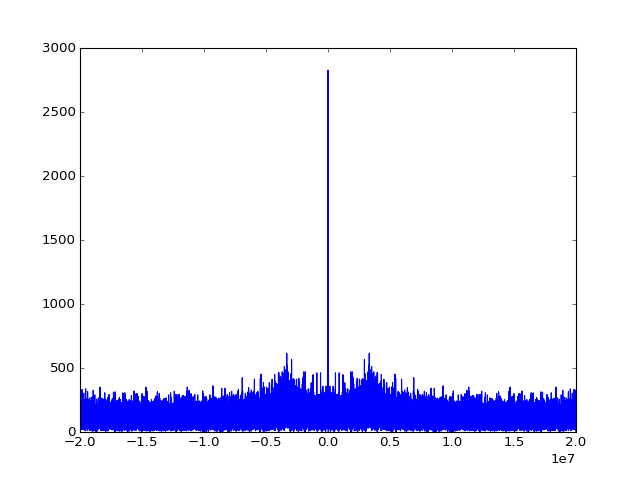
\includegraphics[width=0.5\textwidth]{./figures/noise_fft2.png}}
  \hfill
  \subfloat[Peak at 16.5 kHz]{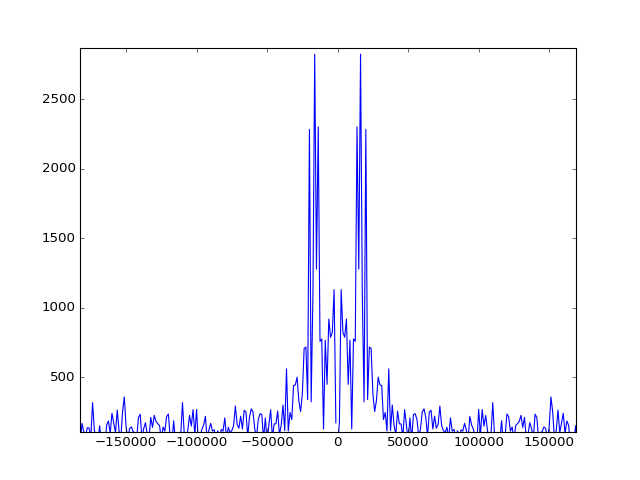
\includegraphics[width=0.5\textwidth]{./figures/noise_fft.png}}
  \caption{Noise Spectrum (ATCA+FEE+PMT).}
  \label{fig:noise}
\end{figure}


\section{FEE modeling for simulation}
Once the design has been validated through real measurements it is of main importance to build a simulation model which can help in the development of other parts of the project. This time the model has a high level of abstraction in order to be easily integrated with the software analysis modules, Python language with help of Numpy-Scipy libraries has been chosen as the tool to build it.
\subsection{Simple FEE model}
A first approach to the FEE model was done by using only a first order high pass filter followed by a fourth order low pass filter (due to LT6600) with the right gain factor. This is basically the model shown in fig. \ref{fig:fig_FEE_full} where the amplifier has a fourth order low-pass response. The frequency response is shown in fig. \ref{fig:FEEsimple_freq}. The noise is introduced in the system to resemble the noise behavior of the real system, taking into account the filtering effect of every part. This is to say that for instance, the input equivalent noise of the FEE has been increased to shown its right effect given the 3 MHz bandwidth. The noise equivalent model of the FEE is shown in fig. \ref{fig:noise_eq} as well as the noise equations relative to the different noise contributions



\begin{align}  
  GAIN &= FEE_{GAIN}.DAQ_{GAIN} \\ 
  vo_{TOTAL_{noise}}^{2} &= v_{DAQnoise}^{2}(out) + v_{FEE+PMBnoise}^{2}(out) \\
  vo_{TOTAL_{noise}}^{2} &= \int_{0}^{BW=3MHz}{v_{FEE+PMBnoise}^{2}.{\lvert}GAIN.H(jw){\rvert}^2}  \\
  & + \int_{0}^{BW=20MHz}{v_{DAQnoise}^{2}.{\lvert}DAQ_{GAIN}.H(jw){\rvert}^2}\\
  vo_{TOTAL_{noise(rms)}} &= \sqrt{vo_{TOTAL_{noise}}^{2}} = 0.76LSB_{rms}  
\end{align}


\begin{figure}
  \begin{center}
    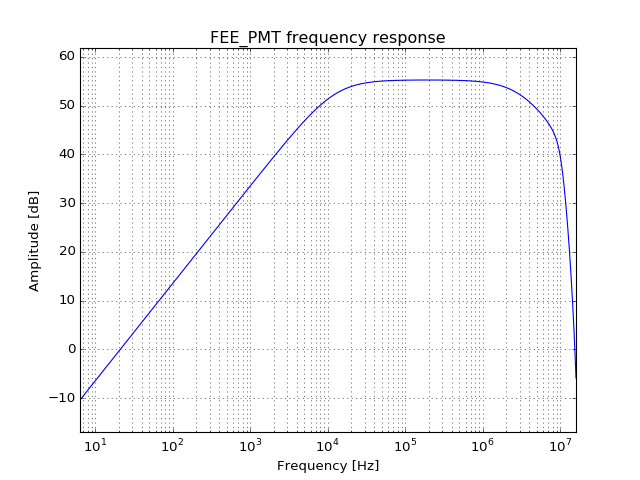
\includegraphics[width=0.7\textwidth]{./figures/FEEsimple_freq.png}
    \caption{}
    \label{fig:FEEsimple_freq}
  \end{center}
\end{figure}

\begin{figure}
  \begin{center}
    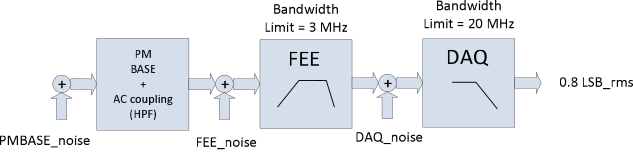
\includegraphics[width=\textwidth]{./figures/NOISE.png}
    \caption{}
    \label{fig:noise_eq}
  \end{center}
\end{figure}

\subsection{Full FEE model}
However the simple model fails modeling the PMT base interaction as the PMT base capacitors can exchange some charge with the coupling capacitor. Using an equivalent circuit shown in fig. \ref{fig:FEE_PMT} (left) which can be even further simplified in \ref{fig:FEE_PMT} (right) the equations shown in eq.\ref{eq:full_fee} arise. 

\begin{figure}[!tbp]
  \centering
  \subfloat[FEE Full Model ]{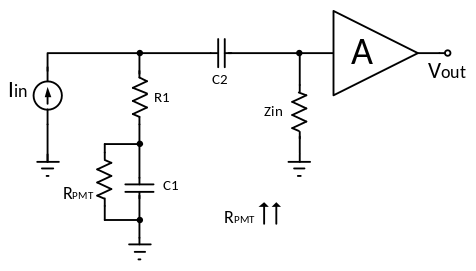
\includegraphics[width=0.5\textwidth]{./figures/FEE_PMT.png}}
  \hfill
  \subfloat[FEE Full Model Simplified]{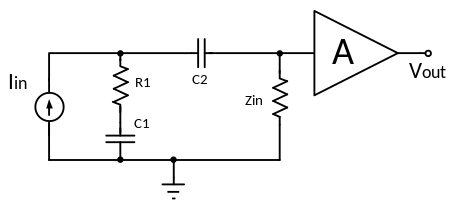
\includegraphics[width=0.5\textwidth]{./figures/FEE_PMT_simple.png}}
  \caption{FEE Full model.}
  \label{fig:FEE_PMT}
\end{figure}

\begin{align}
\frac{v_O}{i_I} &= \frac{Z_{in}}{(1+\frac{C_1}{C_2})}\frac{1+R_1C_1s}{1+\frac{(R_1+Z_{in})C_1}{(1+\frac{C1}{C2})}s} \label{eq:full_fee}\\ 
\frac{v_O}{i_I} &= \frac{Z_{in}}{(1+\frac{C_1}{C_2})}.\frac{1}{1+\frac{(R_1+Z_{in})C_1}{(1+\frac{C_1}{C_2})}s}+\frac{R_1R_2}{R_1+Z_{in}}.\frac{\frac{(R_1+Z_{in})C_1}{1+\frac{C_1}{C_2}}s}{1+\frac{(R_1+Z_{in})C_1}{1+\frac{C_1}{C_2}}s}
\end{align}

The noise is introduced exactly the same way as before. Spice simulations where carried out in order to check the model at low frequencies including the base connection. The results shown in fig. \ref{fig:FEE_check} validate the model that includes the low frequency zero that generates a small amount of low frequency distortion. The same situation happens with the high $\tau$ solution when $R_{par}$ is considered though the amount of distortion is much higher in this latter case. 

\begin{figure}[!tbp]
  \centering
  \subfloat[FEE Full freq. response ]{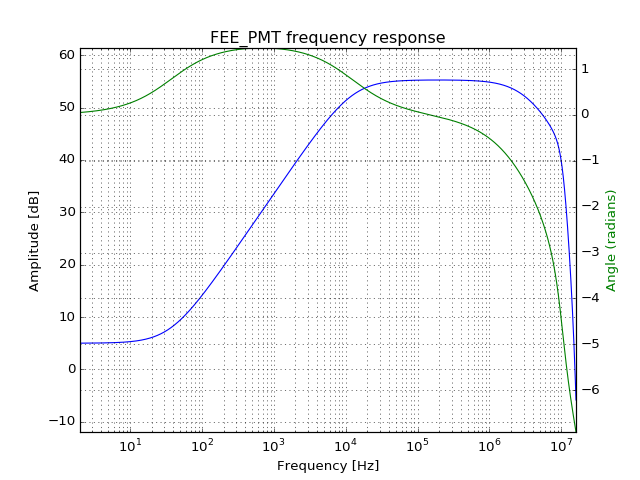
\includegraphics[width=0.5\textwidth]{./figures/FEEfull_freq.png}}
  \hfill
  \subfloat[SPICE simulated FEE]{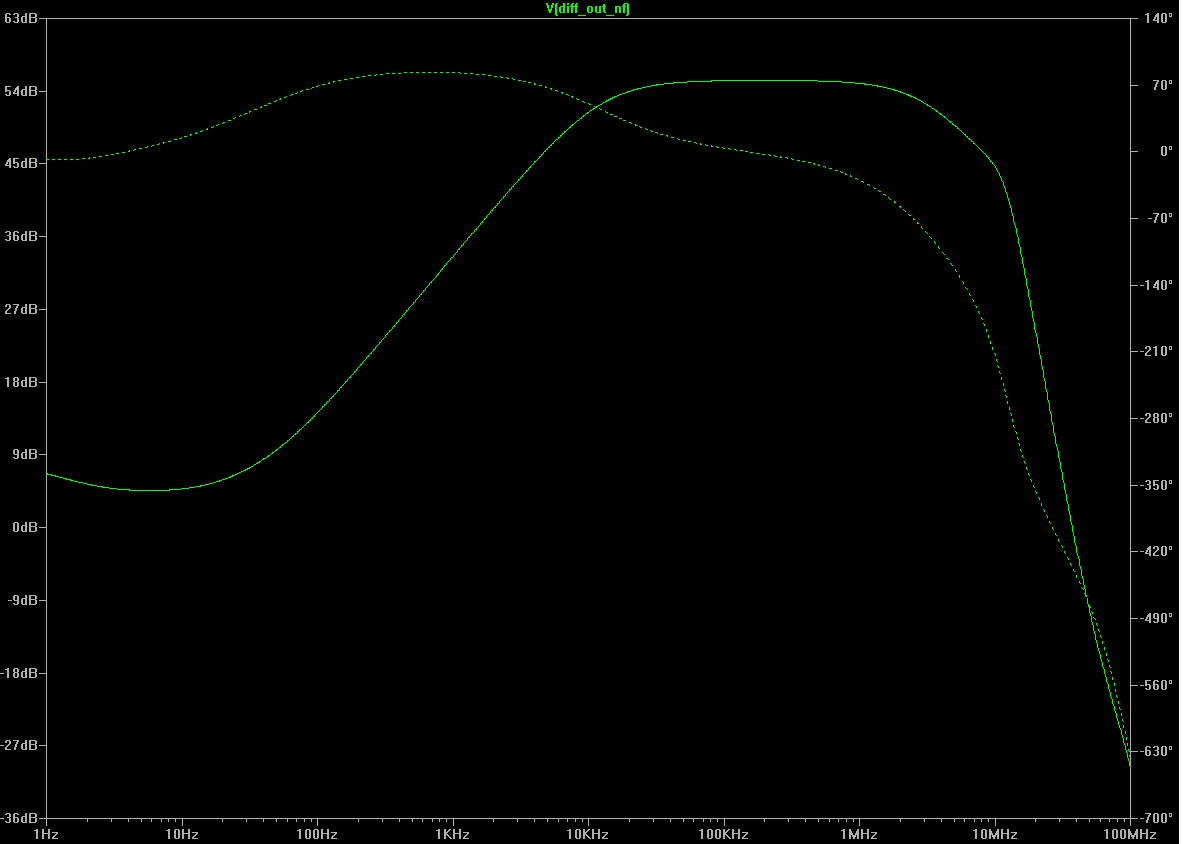
\includegraphics[width=0.5\textwidth]{./figures/FEE_PMT_freq_response_simulated_spice.png}}
  \caption{FEE model check.}
  \label{fig:FEE_check}
\end{figure}

\par As we will see later on, the low frequency behavior can be corrected using a digital post-processing high pass filter that nullifies that low frequency zero. This will help attenuating low frequency noise and distortion.

\section{Digital Baseline Restoration}
\par As explained before, the design trade-off taken with this solution allowed a more relaxed FEE design, less prone to low frequency issues and less noisy in general relying on a Digital Signal Postprocessing (DSP) to recover the baseline distortion introduced by the AC coupling capacitor. In order to design the DSP algorithm the inverse function of the high pass filter (HPF) of order 1 was obtained. It has a very simple impulse response structure composed of a delta in the origin plus a step function whose amplitude equals the value of $\frac{1}{\tau}$ where $\tau$ is $(R_1+Z_{in}).C$. This means that the convolution operation can be carried out using just an accumulator and a multiplier instead of a FIR filter.     

\begin{figure}[!tbp]
  \centering
  \subfloat[HPF Inverse impulse response ]{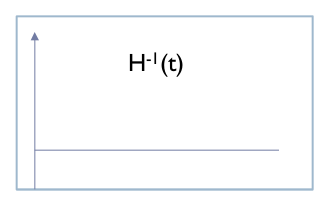
\includegraphics[width=0.5\textwidth]{./figures/Impulse_R.png}}
  \hfill
  \subfloat[MAC implementation]{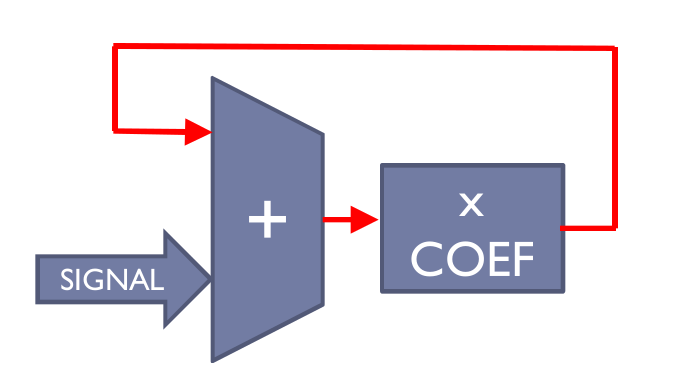
\includegraphics[width=0.5\textwidth]{./figures/Impulse_MAC.png}}
  \caption{Inverse HPF Implementation.}
  \label{fig:FEE_check}
\end{figure}

\par An interesting advantage of this algorithm is that it doesn't have to work continuously, it only has to be activated when a pulse is detected and can be switched off when the pulse ends. This means that an important amount of low frequency noise filtered by the AC coupling capacitor will not be restored since it is slower than the pulse length. Figure \ref{fig:BLR_algo} shows a simple version of the BLR algorithm.


\begin{figure}[!tbp]
  \centering
  \subfloat[Basic Algorithm of Digital BLR]{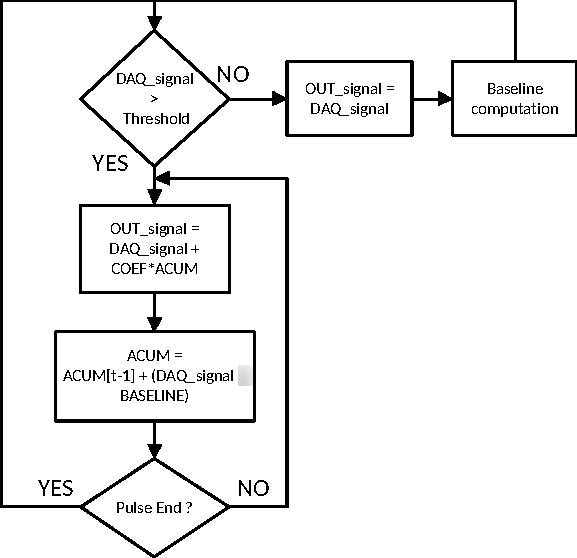
\includegraphics[width=0.55\textwidth]{./figures/BLR_algo.pdf}}
  \hfill
  \subfloat[Basic Algorithm with Cleaning Filter]{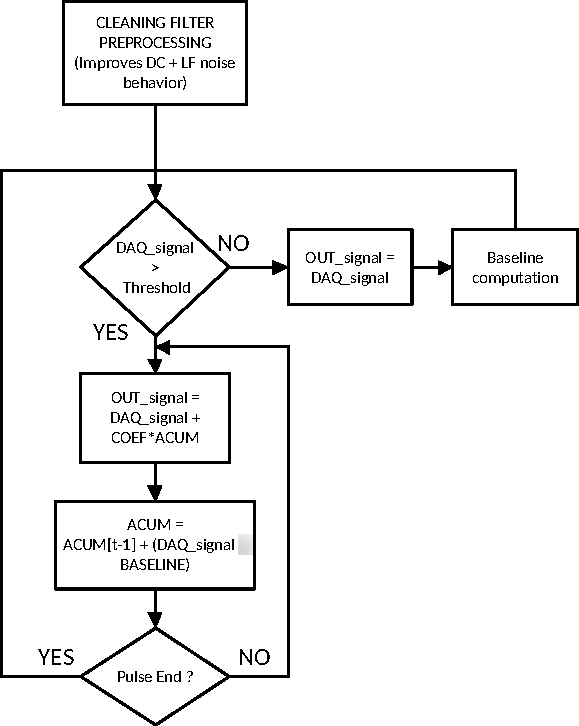
\includegraphics[width=0.425\textwidth]{./figures/BLR_algo2.pdf}}
  \caption{Basic Alg. and Cleaning Filter improvement}
  \label{fig:BLR_ralgo}
\end{figure}



Simulation results with the FEE model show that the algorithm works as expected but there is a small difference in the baseline height when the pulse ends (fig. \ref{fig:BLR_results}). This small error is due to the low frequency zero which introduces a low amount of DC in the theoretically AC coupled output signal of the FEE.

\begin{figure}[!tbp]
  \centering
  \subfloat[Square Pulse reconstruction]{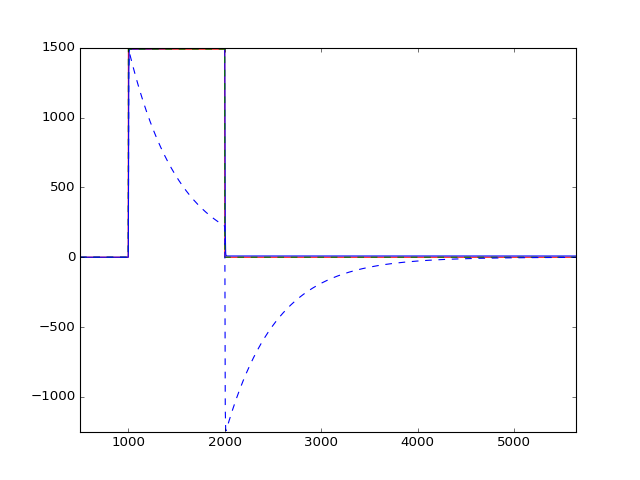
\includegraphics[width=0.5\textwidth]{./figures/BLR_simple_result.png}}
  \hfill
  \subfloat[Baseline error]{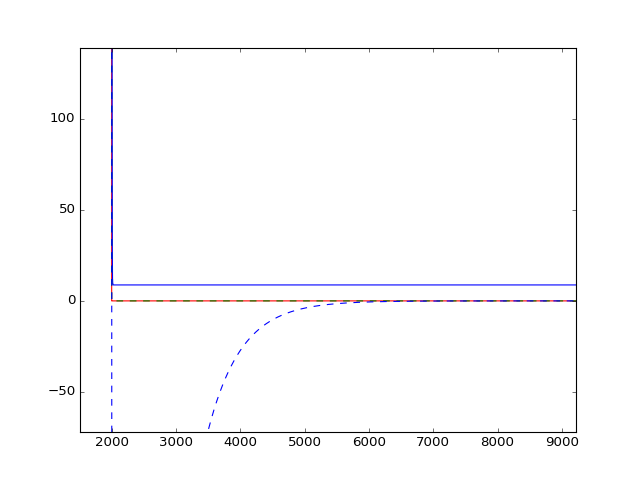
\includegraphics[width=0.5\textwidth]{./figures/BLR_simple_result2.png}}
  \caption{Noiseless square pulse reconstruction}
  \label{fig:BLR_results}
\end{figure}

\par If the DAQ output signal is filtered by a high pass filter whose cutoff frequency is the same as the low frequency zero of the FEE the effect is completely corrected and the reconstructed signal shows no baseline shift at the end (fig. \ref{fig:BLR_filt}. This "cleaning filter" is applied before the BLR operation and doesn't interfere with its behavior. 

\begin{figure}
  \begin{center}
    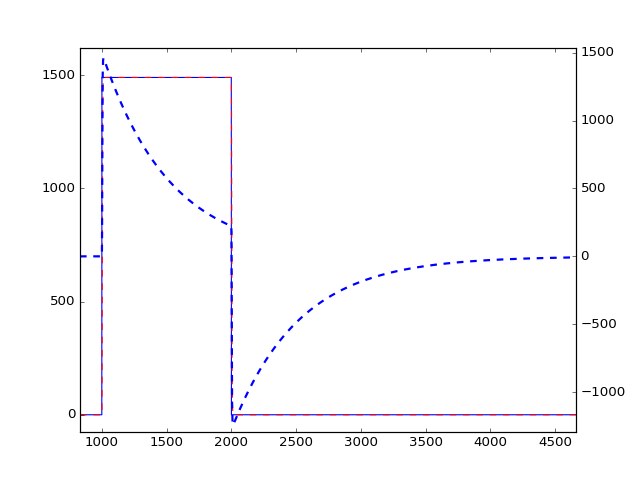
\includegraphics[width=0.5\textwidth]{./figures/BLR_filt.png}
    \caption{BLR Reconstruction after Cleaning Filter}
    \label{fig:BLR_filt}
  \end{center}
\end{figure}


\subsection{Noise effects on BLR}
Since the BLR algorithm uses an accumulator, it might be sensitive to noise and its effects must be studied not only as simple noise equivalent but also taking into account the effect of different frequency components. First of all the coefficient applied to the accumulator will have an strong effect. Although it is already fixed by previous design trade-offs there is still room for some fine tunning if needed. Figure \ref{fig:BLR_noise} shows the results for a worst case signal with added noise and the statistics for 2000 MC noise runs. 
\par However the noise introduced at the simulation models has a zero mean gaussian profile. If the noise has a non zero mean, the accumulator might get in trouble.  In a typical ideal pulse, the accumulator should end the deconvolution process in an empty state. Sometimes a small residue remains in the accumulator after the process but it shouldn't be dangerous if the residue is random. However due to finite sampling of the signals the residue is not always random. For instance in a burst of  short signals (photoelectrons) processing the residue tends to be positive because the pulses have a higher positive lobe. As a consequence the accumulator starts to rise without limit introducing a baseline shift in the output signal (fig. \ref{fig:BLR_error} red signal accumulator and blue reconstructed).


\begin{figure}[!tbp]
  \centering
  \subfloat[Worst Case signal]{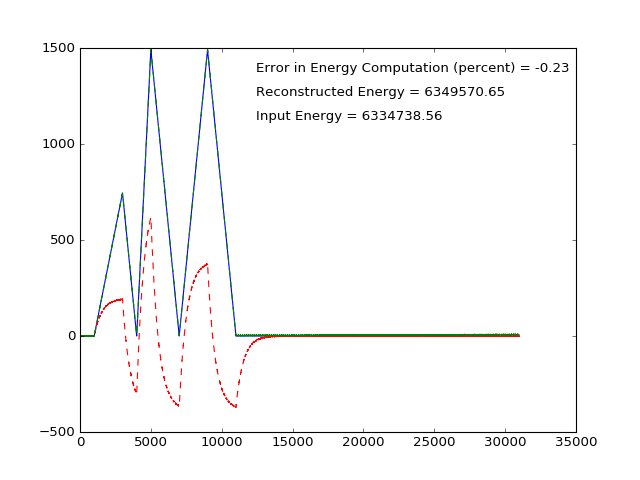
\includegraphics[width=0.5\textwidth]{./figures/BLR_noise.png}}
  \hfill
  \subfloat[Energy Resolution Statistics]{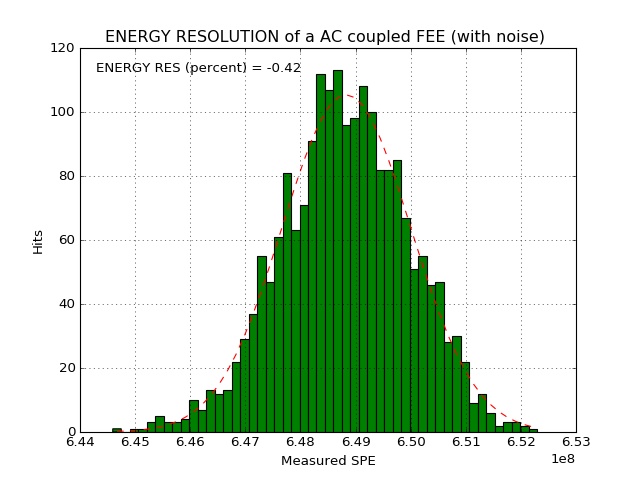
\includegraphics[width=0.5\textwidth]{./figures/BLR_noise2.png}}
  \caption{Noisy worst case signal reconstruction}
  \label{fig:BLR_noise}
\end{figure}

\begin{figure}
  \begin{center}
    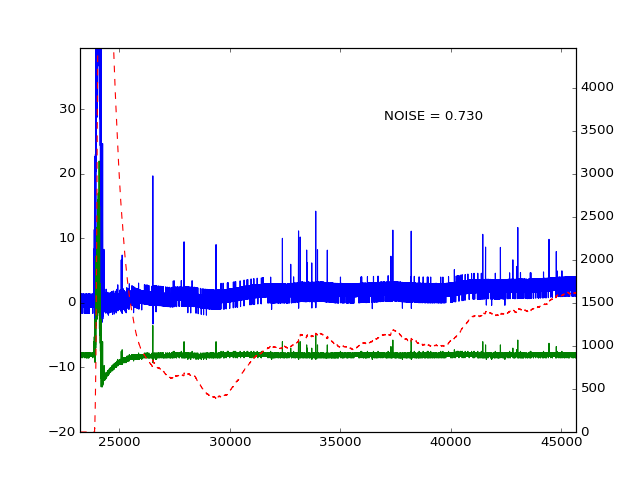
\includegraphics[width=0.7\textwidth]{./figures/BLR_error1.png}
    \caption{Basic BLR algorithm failure}
    \label{fig:BLR_error}
  \end{center}
\end{figure}


\section{Accumulator Based Control BLR}
\par As a possible solution to the previous problem a new algorithm has been designed which introduces a control mechanism based on a smooth mechanism to deplete the residue remaining in the accumulator after a pulse reconstruction. The algorithm flowchart is shown in fig. \ref{fig:BLR_acc_algo}. The first difference is that in this algorithm the reconstruction process is started independently from the pulse start, and can be even working forever. The control relies on the accumulator operations that can be Update or Discharge. When the DAQ signal rises above a  threshold or the accumulator value is above another threshold (which is the condition for an active pulse) the accumulator is updated as in the original algorithm. However when none of those conditions are met, which means that there is no active signal pulse, the accumulator is forced to a controlled discharge state. This discharge operation is carried out following a smooth curve so that the reconstructed signal shows no jumps or discontinuities. Figure \ref{fig:BLR_error_acum} shows the behavior of this new algorithm in the same situation where the original one failed to recover the baseline.


 \begin{figure}
  \begin{center}
    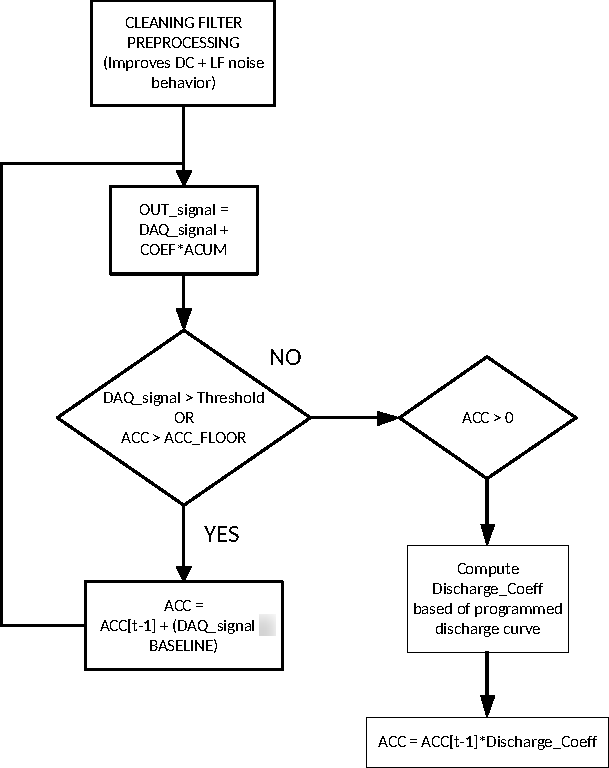
\includegraphics[width=0.8\textwidth]{./figures/BLR_acc_algo.pdf}
    \caption{Accumulator based BLR}
    \label{fig:BLR_acc_algo}
  \end{center}
\end{figure}


\begin{figure}
  \begin{center}
    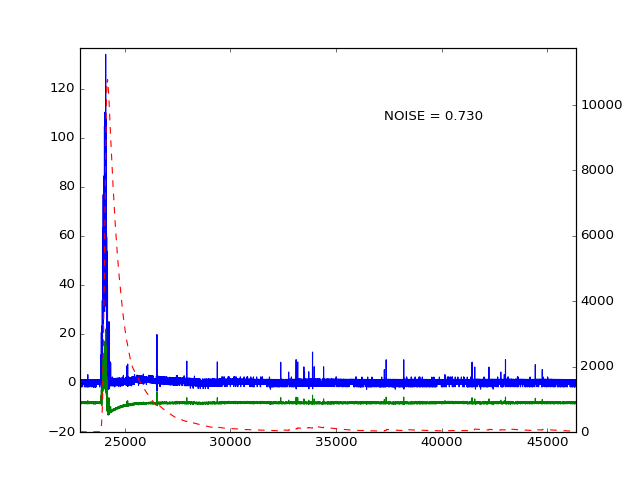
\includegraphics[width=0.8\textwidth]{./figures/BLR_error_acum.png}
    \caption{Improved Accumulator Based BLR}
    \label{fig:BLR_error_acum}
  \end{center}
\end{figure}


\end{document}
